\documentclass[12pt]{article}

%% preamble: Keep it clean; only include those you need
\usepackage{amsmath}
\usepackage[margin = 1in]{geometry}
\usepackage{graphicx}
\usepackage{booktabs}
\usepackage{natbib}

% for space filling
\usepackage{lipsum}
% highlighting hyper links
\usepackage[colorlinks=true, citecolor=blue]{hyperref}

\usepackage{hyphenat}
\hyphenation{word-list} %

%% meta data

\title{Impact of diet on chronic kidney disease}
\author{SHIYI PENG\\
  Department of Statistics\\
  University of Connecticut
}

\begin{document}
\maketitle

\begin{abstract}

Healthy dietary patterns are associated with a lower risk of Chronic Kidney Disease. More research is needed into the effects of specific food groups and beverages on kidney function\cite{van2020diet}.

\end{abstract}


\section{Introduction}
\label{sec:intro}

Chronic Kidney Disease is a global health burden that increases the risk of premature death or reduced quality of life. However, Chronic Kidney Disease does not present with obvious symptoms until the later stages of the disease.Therefore,it is easy to ignore Chronic Kidney Disease until it becomes end stage renal disease, which requires dialysis or kidney transplant for whole life. We need to know how to protect our kidneys in our daily lives and how to slow down the progression of chronic kidney disease. Carbonated drinks and sugar-free beverages are now popular among young people, so it is important to know whether such drinks are harmful to the kidneys. Also everyone should consume a certain amount of carbohydrates every day, however few studies have investigated the effect of carbohydrate intake on Chronic Kidney Disease patients,so another part of the article will be centered on carbohydrate intake\cite{hill2016global}

% roadmap
The rest of the paper is organized as follows.
The data will be presented in Section~\ref{sec:data}.
The methods are described in Section~\ref{sec:meth}.
The results are reported in Section~\ref{sec:resu}.
A discussion concludes in Section~\ref{sec:disc}.


\section{Data}
\label{sec:data}
\begin{equation}
  IQR=Q3-Q1
\end{equation}
$IQR$ is the interquartile range contains the second and third quartiles, or the middle half of your data set. 

\section{Methods}
\label{sec:meth}

Use this section to present the methodologies that will generate results by analyzing the data. Suppose that in eGFR 0-59mL·/min·1.73m2 group, the mortality risk was lower in participants who had 30-45\% energy from carbohydrate (average HR 0.68, 95\%CI 0.51-0.90, compared with 60\%), 5\%-20\% energy from sugar (average HR 0.64, 95\%CI 0.48-0.87, compared with 40\%), 40-50\% energy from non-sugar carbohydrate (average HR 0.58, 95\%CI 0.39-0.85, compared with 30\%). 



\begin{equation}
eGFR = 175 x (SCr)^(-1.154) x(age)^(-0.203) xSex[male=1,female=1.75] x1.212 [if Black]
\end{equation}

which states that $eGFR$ is estimated glomerular filtration rate (mL/min/1.73 m\^2),$Scr$ is standardized serum creatinine( mg/dL), $age$ is years.



\section{Results}
\label{sec:resu}

Non-linear associations were found between the macronutrients and all-cause mortality risk in CKD patients. Low carbohydrate intake reduces the all-cause mortality risk. Moreover, the different effects of the carbohydrate constituents on all-cause mortality risk were observed in this study. Non-sugar carbohydrates reduced the mortality risk while sugar increased the mortality risk. Thus, dietary advice should be given according to the current diet structure (especially the percentage of carbohydrate intake) and sugar/non-sugar carbohydrates should be considered when adjusting the carbohydrate intake in CKD patients.

\vspace{\baselineskip}
\vspace{\baselineskip}
\begin{tabular}{|l|l|l|l|l||l|}
\hline
     & Quantile1 & Quantile12 & Quantile3 & Quantile4 & p-trend* \\ 
\hline
    Carbohydrate & 1 & 1.14 (0.89-1.45) & 1.23 (0.98-1.54) & 1.35 (1.05-1.72) & 0.014 \\ 
  Sugar & 1 & 0.91 (0.70-1.17) & 1.00 (0.81-1.24) & 1.27 (1.00-1.61) & 0.030\\ 
\hline
\end{tabular}
\vspace{\baselineskip}

Figure~\ref{fig:111} Association between low carbohydrate/sugar diet and all-cause mortality by quantiles in participants with CKD.


\begin{figure}[tbp]
  \centering
  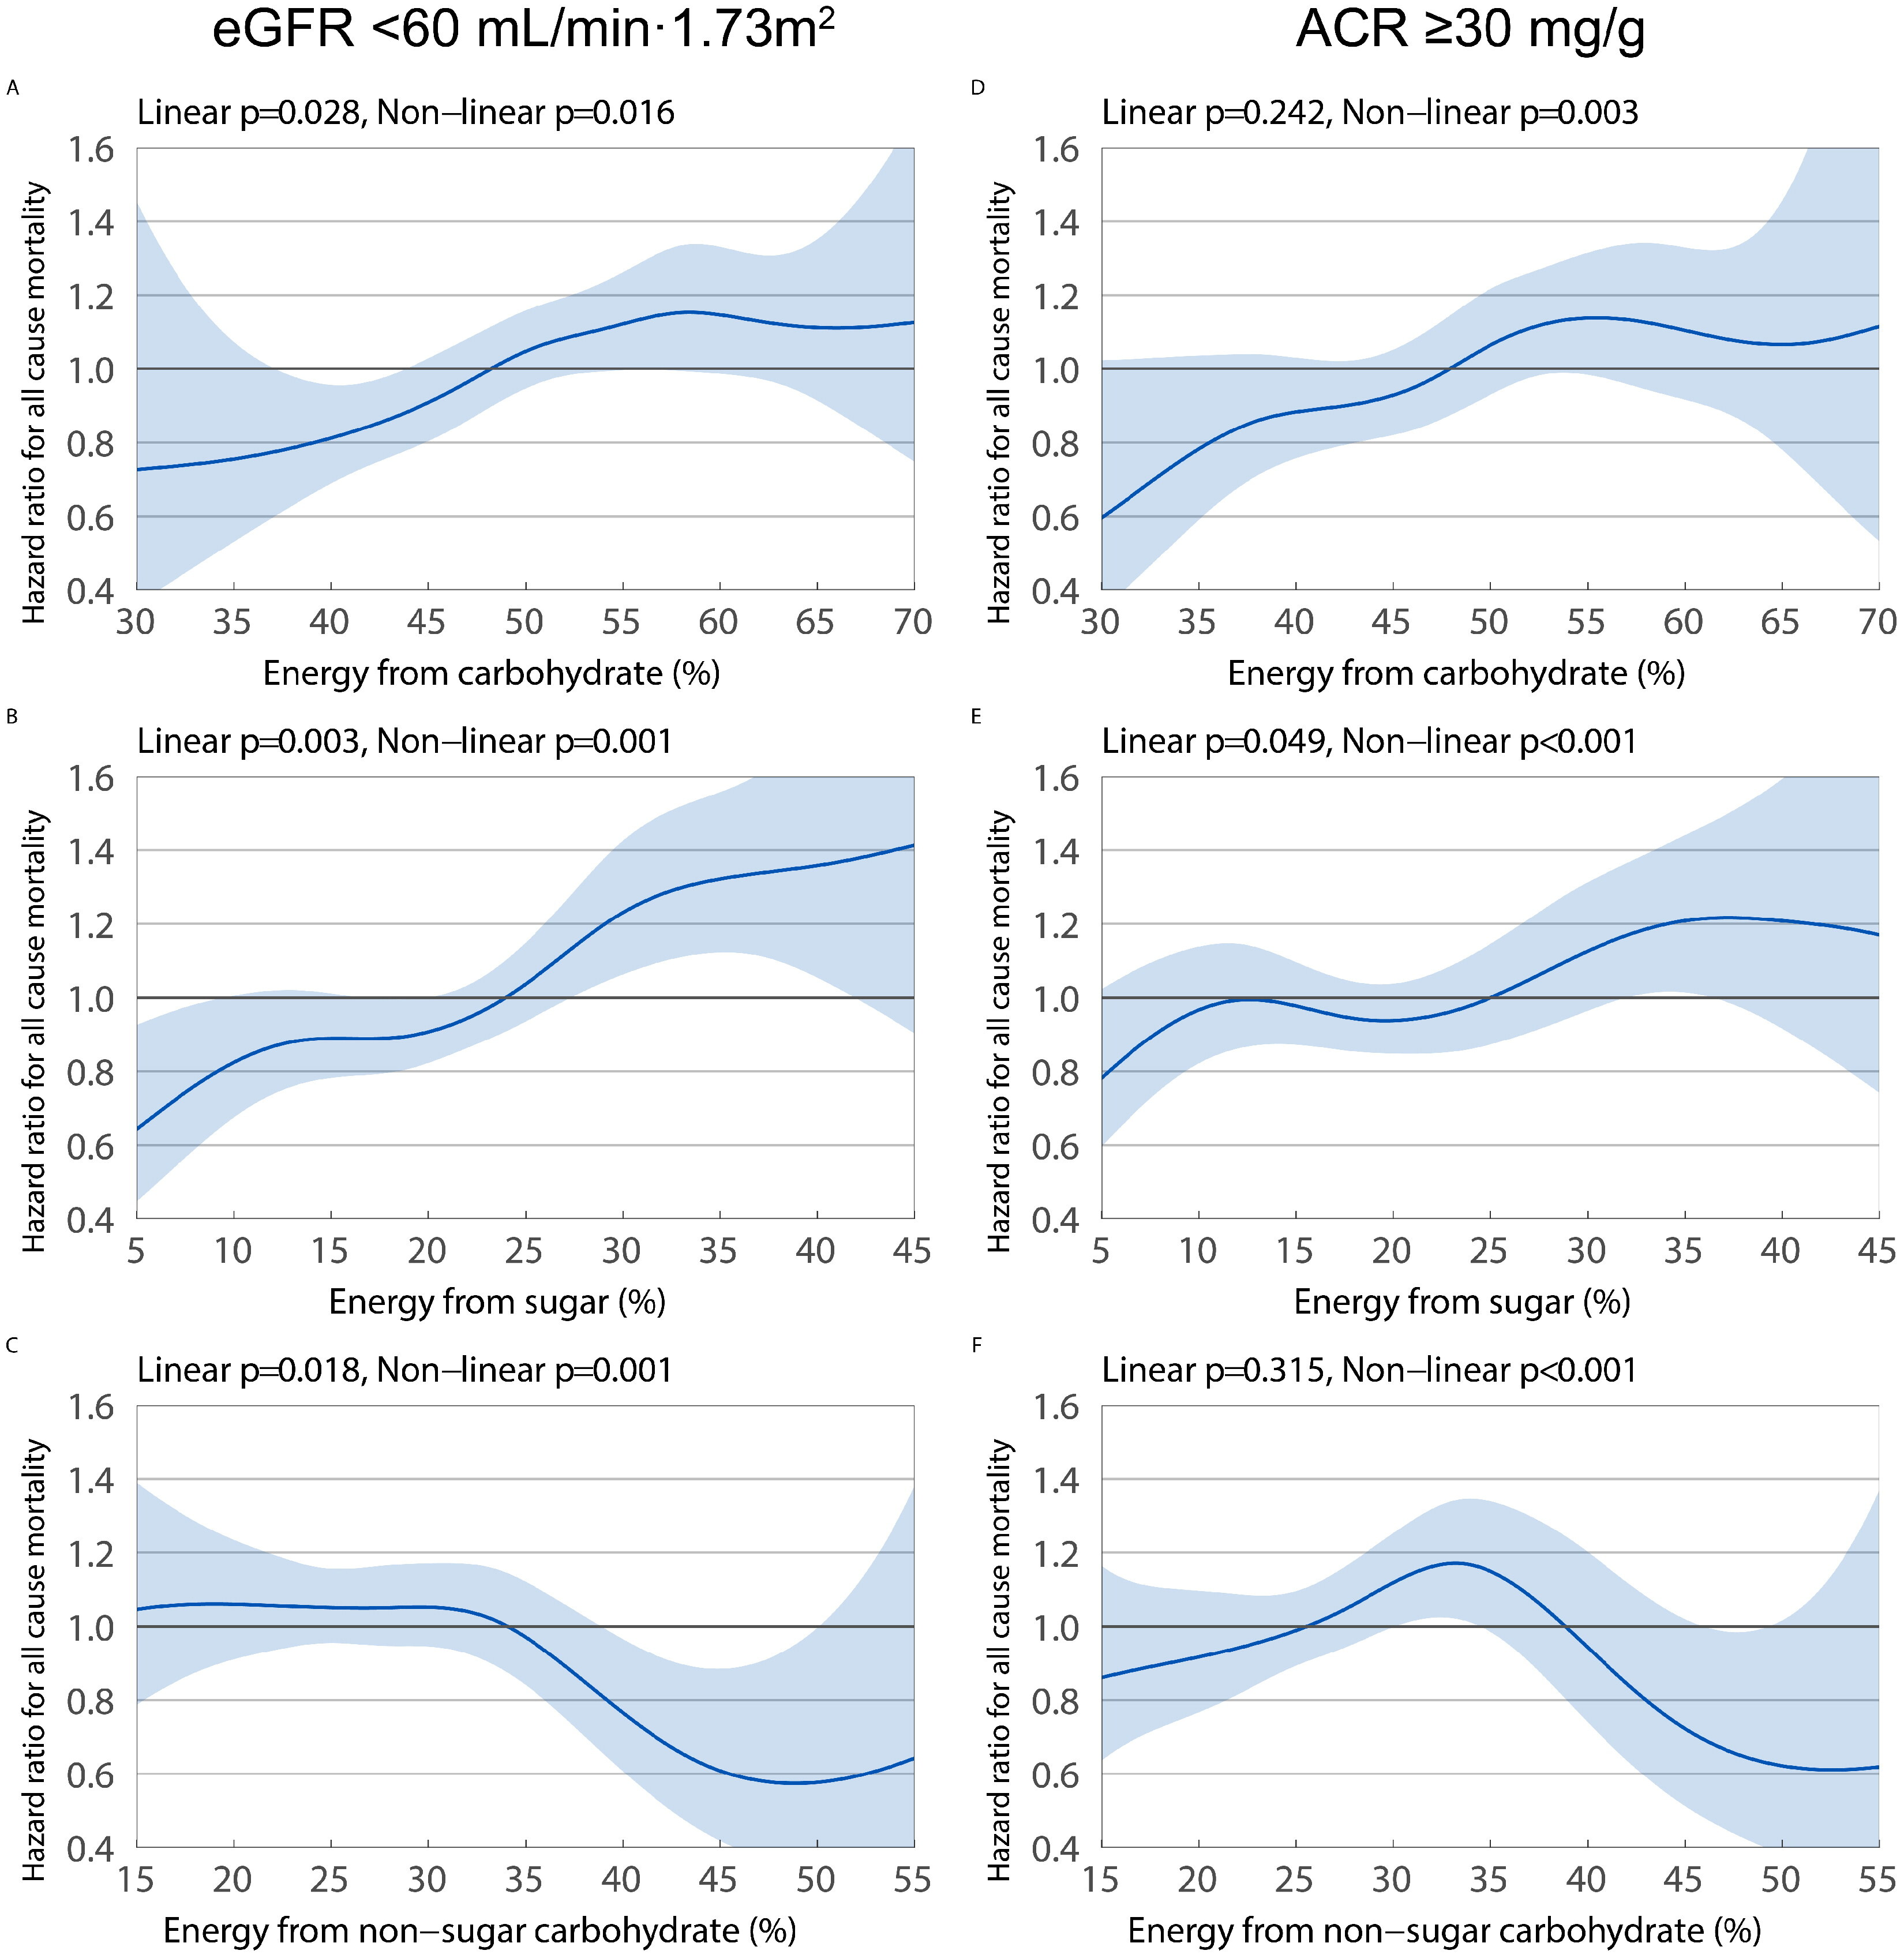
\includegraphics[width=\textwidth]{111.jpg}
  \caption{This is my first figure.}
  \label{fig:111}
\end{figure}

\section{Discussion}
\label{sec:disc}

We explored specific components and different sources of macronutrients (e.g., sugar, fiber, saturated fat, animal protein) and how the changes in diet pattern would affect the risk of mortality by replacing the carbohydrate or sugar with other macronutrients using the iso-caloric replacement method. However, this study has several limitations. First, non-sugar carbohydrate was calculated by subtracting sugar from carbohydrates to represent the starch because no available information was provided in NHANES dietary data. Second, the iso-caloric replacement is based on the inter-participants comparison and might not represent the diet changes of the individual in actual daily life. Third, the selection bias is possible since the dietary data were all from NHANES and might not represent the population other than US adults. Fourth, as an observational study, causality could not be determined.The effect of a high protein diet in CKD patients remained controversial, and more long-term and extensive sample-size studies are required\cite{ren2023associations}.

\bibliographystyle{plain}
\bibliography{Ref}
\end{document}
